\documentclass[12pt,a4paper]{article}
\usepackage[utf8]{inputenc}
\usepackage{amsmath}
\usepackage[brazilian]{babel} % Brazil or not Brazil??
\usepackage{amsfonts}
\usepackage{amssymb}
\usepackage{graphicx}
\usepackage[margin=0.8in]{geometry}


\begin{document}
\title{\vspace{70mm}\Huge Experimento 06 - Calorimetria}
\author{ Giovani Garuffi\qquad\hfill
		\textit {RA: 155559}\protect\\
		João Baraldi\hfill
		\textit{RA: 158044}\protect\\
		Lauro Cruz\hfill
		\textit{RA: 156175}\protect\\
		Lucas Schanner\hfill
		\textit{RA: 156412}\protect\\
		Pedro Stringhini\hfill
		\textit {RA: 156983}								
		}
\maketitle
\newpage
\section{Resumo}


\section{Objetivos}


\section{Procedimento Experimental e Coleta de Dados}


\subsection{Procedimento}



\subsection{Dados Obtidos}

A Tabela \ref{dados} apresenta as medições Da tensão medida no termopar, em função da temperatura.

\begin{table}[!htbp]

\centering
\def\arraystretch{1.5}
\caption{Dados obtidos no experimento}

\begin{tabular}{|r|r|}
\hline
Tensão $(mV)$ & Temperatura $(C)$\\
\hline
 4.62 & 89 \\
 \hline
 4.40  & 87 \\
 \hline
 4.19 & 84 \\
 \hline
 3.96 & 80 \\
 \hline
 3.82 & 78 \\
 \hline
 3.04 & 65 \\
 \hline
 2.89 & 62 \\
 \hline
 2.44 & 54 \\
 \hline
 2.31 & 51 \\
 \hline
 2.03 & 47 \\
 \hline
 1.94 & 45 \\
 \hline
 1.80  & 42 \\
 \hline
 1.69 & 40 \\
 \hline
 1.44 & 37 \\
\hline
\end{tabular}

\emph{O erro na temperatura é de $0.5 C$, e na tensão de $0.01 mV$}
\label{dados}
\end{table}




\section{Análise dos Resultados e Discussões}
\subsection{Curva de Calibração do Termopar}
Para comparar os dados obtidos no experimento e os dados conhecidos de tensão em função da temperatura, foi construído o graf \ref{termopar}

\begin{figure}[!htbp]
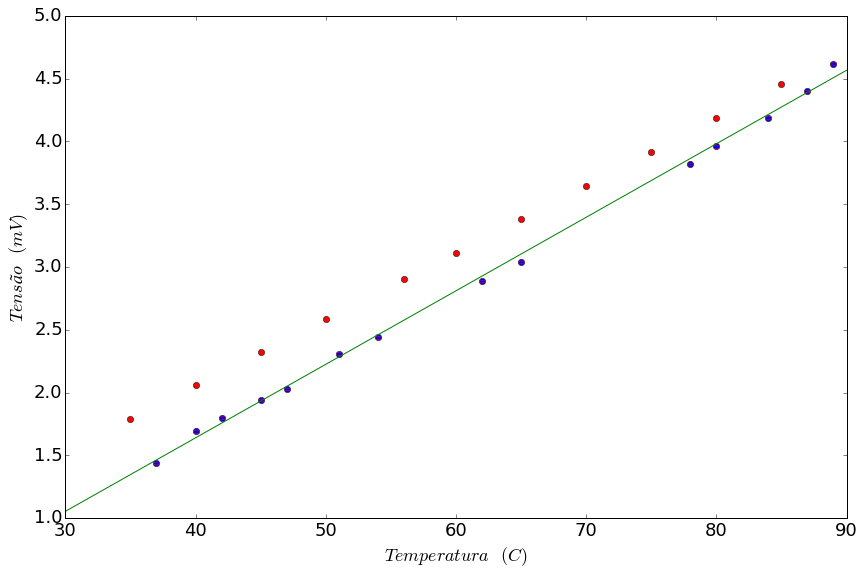
\includegraphics[scale=0.55]{termopar.png}
\label{termopar}
\caption{Curva de calibração do termopar. As medidas Azuis são as obtidas experimentalmente e as vermelhas são as esperadas}
\end{figure}


\section{Conclusões}



\end{document}

